%
% File ccl2020-zh.tex
%
% Contact: zhangyue@westlake.edu.cn
%%
%% Based on the original version of COLING-2018 file (coling2018.tex), with changes made by Yue Zhang.
%%

\documentclass[11pt]{article}
\usepackage{graphicx} %插入图片的宏包
\usepackage{float} %设置图片浮动位置的宏包
\usepackage{subfigure} %插入多图时用子图显示的宏包
\usepackage[utf8]{inputenc}
\usepackage[hyperref]{ccl2020-zh}
\usepackage{url}
\usepackage{latexsym}
\usepackage{CJKutf8}
\usepackage{indentfirst}
\usepackage{fancyhdr}

\pagestyle{fancy}
\fancyhf{}
\lhead{\begin{CJK*}{UTF8}{gbsn}数据挖掘\end{CJK*}}
\renewcommand{\headrulewidth}{0pt}

%\setlength\titlebox{5cm}

% You can expand the titlebox if you need extra space
% to show all the authors. Please do not make the titlebox
% smaller than 5cm (the original size); we will check this
% in the camera-ready version and ask you to change it back.


\title{数据挖掘大作业————TexTCNN对TNEWS数据分类}

\author{邹世奇 \\
  17123143\\
  {\tt 778377698@qq.com} \\}
  
\date{}


\begin{document}
\begin{CJK*}{UTF8}{gbsn}
\setlength{\parindent}{2em}

\maketitle
\begin{abstract}
  数据挖掘课程大作业,主要使用了PyTorch实现了TextCNN,对TNEWS数据集进行新闻分类工作。
  TextCNN网络结构主要为嵌入层、卷积层、max池化层、全连接层组成。
  在这次大作业中,老师已经基本写好了网络的训练部分。
  因此在训练部分主要是通过单步调试程序, 对TextCNN的训练过程进行学习。
  在了解了TextCNN的工作流程后,自己简单的写了一个测试模块,
  并且最终输出classification\_report代表模型的整体效果的评价。
\end{abstract}

\section{TexTCNN}
\label{intro}

%
% The following footnote without marker is needed for the camera-ready
% version of the paper.
% Comment out the instructions (first text) and uncomment the 8 lines
% under "final paper".
% 

\begin{figure}[H] %H为当前位置,!htb为忽略美学标准,htbp为浮动图形
\centering %图片居中
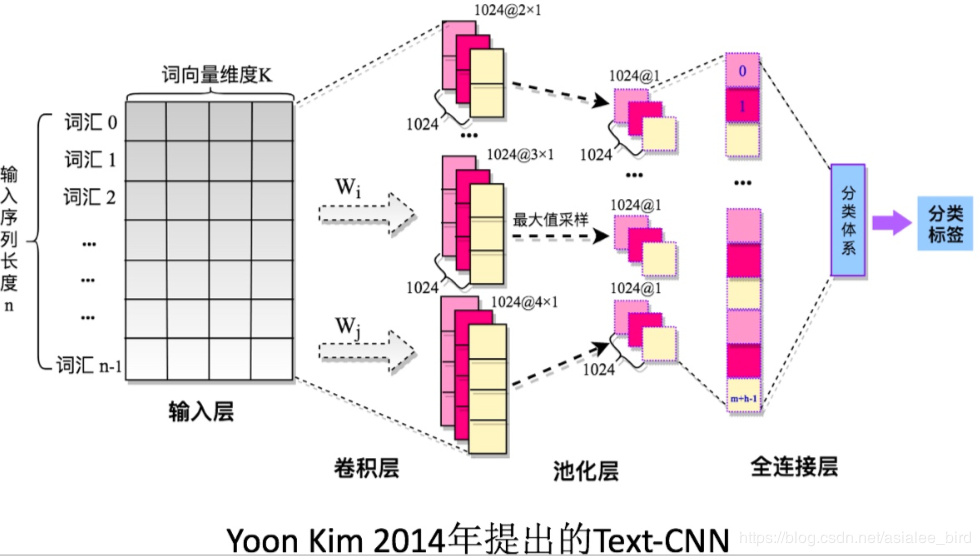
\includegraphics[width=0.7\textwidth]{structure.png} %插入图片,[]中设置图片大小,{}中是图片文件名
\caption{TextCNN结构示意图} %最终文档中希望显示的图片标题
\label{Fig.main2} %用于文内引用的标签
\end{figure}

\subsection{数据预处理}

程序中对数据集构建了三个类,最外层是DataBatchIterator,里面包含DataSet类和Vocab类
DataSet类:即真正地存储数据的类,包含读取数据的方法和相关数值化处理。
Vocab类:字词和标签对数值的映射表类,内含{字词:数值},{数值:字词}字典,以及字词的频率统计字典。

读取数据时,DataSet类按行读取数据集中的词组和标签。而DataBatchIterator类利用DataSet数据,构建Vocab。其中因为min\_freq的设置,
筛选出所有频率大于5的字词,并且按出现的先后顺序构建对数值的映射关系。标签映射表的制作也是同理。

获取映射表后,即可将原DataSet数据进行数值化,将字词和标签都转换成整数表示,此时我们拥有了数字表示的数据集。

\subsection{输入层和嵌入层}
\label{sect:pdf}

输入层本质上就是二维矩阵表示的数据集,
只不过数据不能用原有的字符形式进行表示,
而是通过数据预处理转换为网络可用的数值向量形式。
预处理阶段我们对所有被筛选出的字符编码为了0~3474。
训练中数据划分为多个batch,每个batch大小为32,即每次每批根据32条数据进行训练,
而且原来非定长的sentence在batch中也被补成了统一长度,因此输入层传给嵌入层的最终是[40,32]的数据矩阵。

输入层的数据矩阵中,每个句子由相应的字的编码组成,而字的编码又在0~3473不等,不易找到句子特征。因此我们还要利用嵌入层处理。这里构造了一个nn.Embedding类,其中字总共有为3474种,想要投影到的特征维度是256。这样我们就将值域范围大难以分析特征的原编码,投影到256的维度中进行再编码,即进行特征抽取的编码处理,有点类似PCA的目标。
这样我们输入层本来是[32,40]的数据,即32个句子,每个句子由40个字编码组成,而嵌入层处理后,每个字编码又有256维的嵌入层编码组成,再加上unsqueeze维度处理,因此数据结构变为了[32,1,40,256]。

当然这里使用是数据词向量是自己制作的,但我查找资料得知其实可以导入别人预训练好的词向量,并且优质的词向量往往可以带来更好的结果。
\subsection{卷积层}
\label{ssec:layout}
卷积是一种常用的数学运算, 它将卷积核和其覆盖范围中的数据进行对应相乘,
然后累加求和,最终将一块矩阵区域的信息提取为一个输出值。因此算是一种数据特征提取的方式。而对于文本处理,我们传给卷积层的数据中每一行代表的是一个字词的向量编码,行数为字词数。即每一整行才拥有这个字的完整信息,所以对行长度上的切割是没有意义的。因此TextCNN卷积核的宽度和词的向量宽度是一样的,而高度一般是(2,3,4)。即通过卷积提取连续2,3,4个词的特征,
这样卷积结果不仅拥有每个词的信息,还一定程度上代表着上下文词间关系。

例如高度为2的卷积核不断向下卷积后,原40维的数值,高度为2可以卷积39次,
因此最终这一个卷积核可以得到39维的卷积特征结果。而因为高度为2的卷积核总共有16个,
因此高度2的最终输出结果是[32,16,39]。
同理高度3,高度4的卷积结果依次是[32,16,38],[32,16,37]。

\subsection{池化层}
因为每个卷积核的高度不一样,携带的特征也不一样,
高度2携带着两个字词之间的关系,高度3则是3个字词之间的关系,
因此要归纳所有卷积信息,需要将每个卷积核的信息进行采样成统一的表达方式。
采样一般是使用采样卷积结果中的最大值,即我们认为最大值最能代表这个卷积结果的特征,
最后将归纳的特征信息传递给下一层进行处理。
因此每一个高度的卷积层的输入数据[32,16,:],都统一成为了[32,16]。

\begin{figure}[H] %H为当前位置,!htb为忽略美学标准,htbp为浮动图形
\centering %图片居中
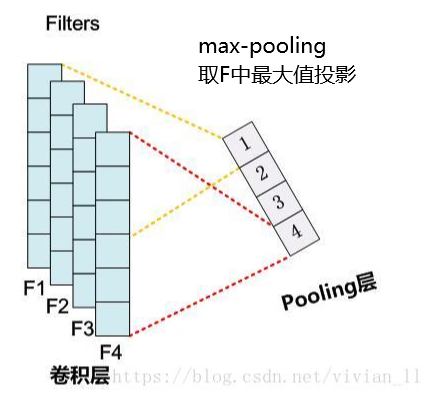
\includegraphics[width=0.7\textwidth]{pooling.jpg} %插入图片,[]中设置图片大小,{}中是图片文件名
\caption{池化层中对卷积层数据的处理} %最终文档中希望显示的图片标题
\label{Fig.main2} %用于文内引用的标签
\end{figure}

\subsection{全连接层}
\label{ssec:first}
将获得的上一层的所有特征信息,进行连接统一,并且将归纳的最终特征映射到标签域中,
实现神经网络的输出。与卷积层相比较,卷积层是抽取局部特征出来,
而全连接层是综合观察所有的局部特征,再次组合成全局整体特征。

例如卷积层输入了三个[32,16]的数据结果,将其顺连接后可以得到[32,3*16]的全特征,
利用这个特征进行全连接层计算。因为标签域为0~15,因此最终输出网络[32,15]的logits结果。

获得logits输出后可以直接使用CrossEntropyLoss进行损失计算,观察网络状态。
并且利用loss进行反向传播计算反馈更新网络,完成网络的训练过程。

\subsection{测试模型}

{\bf 测试过程}: 
首先再次读取之前做好的词汇表和并且读入测试数据集作为DataBatchIterator类用于测试。
这里为了统一训练和测试的框架,我也是仿照使用了batch进行测试集的预测。

载入训练好的模型对输入batch,并且根据每个句子的最大标签值,作为其预测标签而输出。
即输入了32大小的batch,我们可以得到[32]的预测标签数组。

而为了后续对模型结果进行评价方便,这里统一将预测标签和真实标签转换为了list类型,
并且利用了classification\_report函数,生成一个多分类的模型评价报告如下:

\begin{figure}[H] %H为当前位置,!htb为忽略美学标准,htbp为浮动图形
  \centering %图片居中
  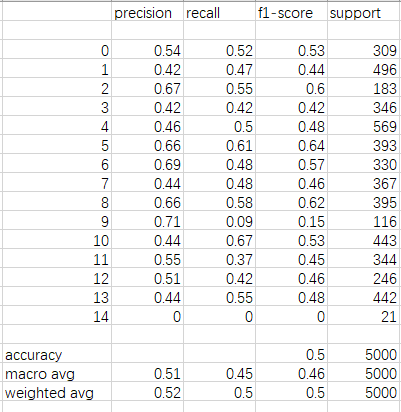
\includegraphics[width=0.7\textwidth]{report.png} %插入图片,[]中设置图片大小,{}中是图片文件名
  \caption{生成的classification\_report表} %最终文档中希望显示的图片标题
  \label{Fig.main2} %用于文内引用的标签
  \end{figure}

{\bf 测试结果}: 
可以看到,总样本数为5000。
精准度,即体现了对于某种预测标签,其中预测正确的比例,可以看出对大多数标签精准度有60\%以上。
召回率,即体现了对于某种真实标签,其中正确识别出该标签的比例,大部分标签也在50\%附近。

值得注意的是,标签9的精准度很高,但是召回率只有0.09,
说明模型没有做出预测为标签9的结果,
可能是样本数量偏差导致。

f1-score和accuracy,即两者的综合评分,最终正确率大概在50\%,
比起完全不依靠模型随机预测的1/15的概率,
通过textCNN的训练效果还是很明显的,当然50\%的效果也不能说很有用。

另外标签14的各项数据都是0,说明对标签14的是识别不太容易,不过这也可能是因为标签14的测试集只有21个样本,
数据不是很具有代表性。
\subsection{学习感想}
这是我第一次进行神经网络的学习,刚接触的时候不知道从哪下手,只知道一些神经网络的理论基本概念。
但运用到程序代码的话,还是不知道怎么去做一个神经网络的框架。而老师写好的网络结构以及网络训练模块,
正好适合我入门。通过单步执行程序,以及阅读众多网上的TextCNN博客,我对神经网络的几大层次有了一定的了解。
并且通过观察数据的格式变换,了解到每一层对数据进行了什么样的处理,想要达成什么样的目的,最终理解TextCNN网络的训练模式。

虽然受限于知识和时间,不能对这个网络进行扩展尝试,最后训练效果也没有很好,但是也算是一次入门级的尝试了。
这次大作业的完成虽然工作量没有很大,但通过对程序的学习理解,还是让我了解到了很多神经网络的相关知识,
希望以后能够在这方面继续深入。

\section*{GitHub地址}
https://github.com/Alobal/DataMining\_TNEWS


% include your own bib file like this:
%\bibliographystyle{ccl}
%\bibliography{ccl2020-zh}

\begin{thebibliography}{}

\bibitem[\protect\citename{}]{}
大规模文本分类网络TextCNN介绍.
\newblock url: 
\newblock https://blog.csdn.net/u012762419/article/details/79561441
\newblock 

\bibitem[\protect\citename{}]{}
pytorch实现textCNN. 
\newblock url: 
\newblock https://doc.flyai.com/blog/textcnn\_pytorch.html
\newblock 

\bibitem[\protect\citename{}]{}
文本分类实战(二)—— textCNN 模型. 
\newblock url:  
\newblock https://www.cnblogs.com/jiangxinyang/p/10207482.html
\newblock 

\bibitem[\protect\citename{}]{}
NLP文本分类入门学习及TextCnn实践笔记(一). 
\newblock url:  
\newblock https://blog.csdn.net/wangyueshu/article/details/106493048
\newblock 

\bibitem[\protect\citename{}]{}
神经网络 优化器 . 
\newblock url:  
\newblock https://www.jianshu.com/p/b88105bb404a
\newblock 

\bibitem[\protect\citename{}]{}
神经网络中Epoch、Iteration相关理解和说明. 
\newblock url:  
\newblock https://blog.csdn.net/program\_developer/article/details/78597738
\newblock 

\bibitem[\protect\citename{}]{}
文本分类实践,TextCNN,实战.
\newblock url:  
\newblock https://www.pythonf.cn/read/81023
\newblock 

\end{thebibliography}

\end{CJK*}
\end{document}

